\documentclass[../_main/handlingar.tex]{subfiles}

\begin{document}
\motion{Tillägg i Policybeslut: Sektionens medaljer och dess utdelning}

Under tidigare år har det funnits diverse medaljer till för sektionsmedlemmarna,
vilket ändrades för några år sen. Däremot ser jag en avsaknad av en medalj där man
representerar E-sektionen men som kan fås (köpas) utan att vara funktionär.

För att åtgärda detta är mitt förslag att införa en E-sektions NolleGasquemedalj,
vilket kan köpas innan Nollegasquen. Eftersom att alla (nollor) som börjar på
sektionen har möjlighet att gå på gasquen så ser jag det som ett ypperligt tillfälle för
dessa att få ett konkret bevis på att de blivit en del av E-sektionen, samt att de har
gått på bal. Annars är enda sättet att få en medalj att bli funktionär, och då får man
inte sin medalj förens efter ett avslutat verksamhetsår som aktiv.

Tanken är att medaljen varje år ska finnas att köpas vid/under nollegasquen, vilken
varje år avslutar nollningen på sektionen. Försäljningen kommer vara öppen både för
nya såväl gamla studenter som går på gasquen, men även besökande sektioner från
andra universitet är välkomna att köpa en medalj.

Anledningen till att jag önskar ett tillskott av en medalj som man ska kunna få utan
att vara funktionär är att jag tycker den kan ses som ett sätt för de som köper den att
visa vilken sektion de tillhör, och också att de har genomfört en hel nollning och varit
på Nollegasquen, vilket är ett väldigt fint event som för många gör att man får upp
ögonen för sektionen.

En medalj är ett sätt att visa sin sektionstillhörighet bland finare event, men också ett
sätt att visa att man har besökt E-sektionen och dess nollning. Vi har redan märken
och pins till de mer ”vardagliga” eventen och medaljen skulle således vara i ett finare
sammanhang.

Själva medaljen skulle jag vilja se utformad med detaljer som ett E, och att det stod
nollegasque på. Själva designen är alltså inte satt än, och det är något som jag vill
utveckla på sikt genom kontakt med företaget där vi innan köpt medaljer. Ett maxpris
per medalj ser jag som \SI{50}{kr}/st inkl. moms i inköpspris, men de kan likväl bli mycket
billigare.

Skulle detta vara lyckat och uppskattat ser jag att det i framtiden skulle kunna läggas
till i budgeten för sigillbevararen.

Jag vill av ovan anledning yrka 
\begin{attsatser}
    \att uppdatera policybeslutet \emph{Sektionens medaljer och dess utdelning} till det bifogade förslaget.
    \att att köpa in 200 stycken sådana medaljer, med ett preliminärt pris på \SI{10108}{kr}, där varje medalj då kommer kosta \SI{50}{kr}/st och frakten är \SI{108}{kr}.
    \att kostnaden belastar utrustningsfonden, samt    
    \att att detta läggs på beslutsuppföljningen till Höstterminsmötet 2019 med undertecknad som ansvarig.
\end{attsatser}

\begin{signatures}{1}
    \mvh
    \signature{Matilda Horn}{Sigillbevarare 2019}
\end{signatures}

\newpage
\section*{Policybeslut: Sektionens medaljer och dess utdelning}

\subsection*{E-sektionens Funktionärsmedaljer}

Sigillbevararen tillsammans med styrelsen avgör vem som gjort sig förtjänt av en funktionärsmedalj. Detta beslut baseras på om personen i fråga fullgjort sitt åtagande i enlighet med reglementet.

\subsubsection*{Funktionärsmedalj 1 år}
En medalj som tilldelas medlemmar som har varit aktiva inom E-sektionen under ett år och utfört sitt funktionärsåtagande.

\subsubsection*{Funktionärsmedalj 3 år}
Ett tillägg på funktionärsmedaljen som tilldelas medlemmar som har varit aktiva inom E-sektionen under tre år och utfört sina funktionärsåtaganden.

\subsubsection*{Funktionärsmedalj 5 år}
Ett tillägg på funktionärsmedaljen som tilldelas medlemmar som har varit aktiva inom E-sektionen under fem år och utfört sina funktionärsåtaganden.

\subsubsection*{Styrelsemedalj}
Till funktionär som har varit styrelseledamot på E-sektionen.

\subsection*{E-sektionens förtjänstmedaljer}
Mottagare av följande medaljer utses av Sigillbevararen tillsammans med styrelsen. Medaljerna ska utdelas på någon av Sektionens högtidligaste sammankomster som till exempel Nollegasquen eller vid Jubileum dit mottagaren av Krusidull-E:t ska bli inbjuden

\subsubsection*{E-sektionens Bidragsmedalj}
Till medlem av sektionen som har bidragit med något till E-sektionen. Medaljen ges till personer som har lagt ner tid för att förbättra eller ge tillbaka något till E-sektionen. Får utdelas till maximalt tre personer per år.

\subsubsection*{E-sektionens Utomstående Förtjänstmedalj}
Medaljen tilldelas individer som ej är sektionsmedlem och som har bidragit något utöver det vanliga.

\subsubsection*{Krusidull-E}
E-sektionens finaste hedersmedalj tilldelas de E-sektionsmedlemar som utöver det vanliga bidragit med utmärkta insatser för E-sektionen. Utdelandet av Krusidull-E ska vara ytterst restriktivt. De personer som utnämns till hedersmedelmar enligt §2.3.2 i stadgarna ska tilldelas Krusidull-E.

\subsection*{\hl{E-sektionens övriga medaljer}}
\subsubsection*{\hl{E-sektionens Nollegasquemedalj}}
\hl{Medaljen finns varje år tillgänglig att köpas av de medlemmar och icke-medlemmar i E-sektionen, vilka kan bestå av nya studenter såväl som besökande universitetsrepresentanter, vilka alla går på Nollegasquen som varje år avslutar nollningen på sektionen.}

\begin{figure}[H]
\begin{center}
    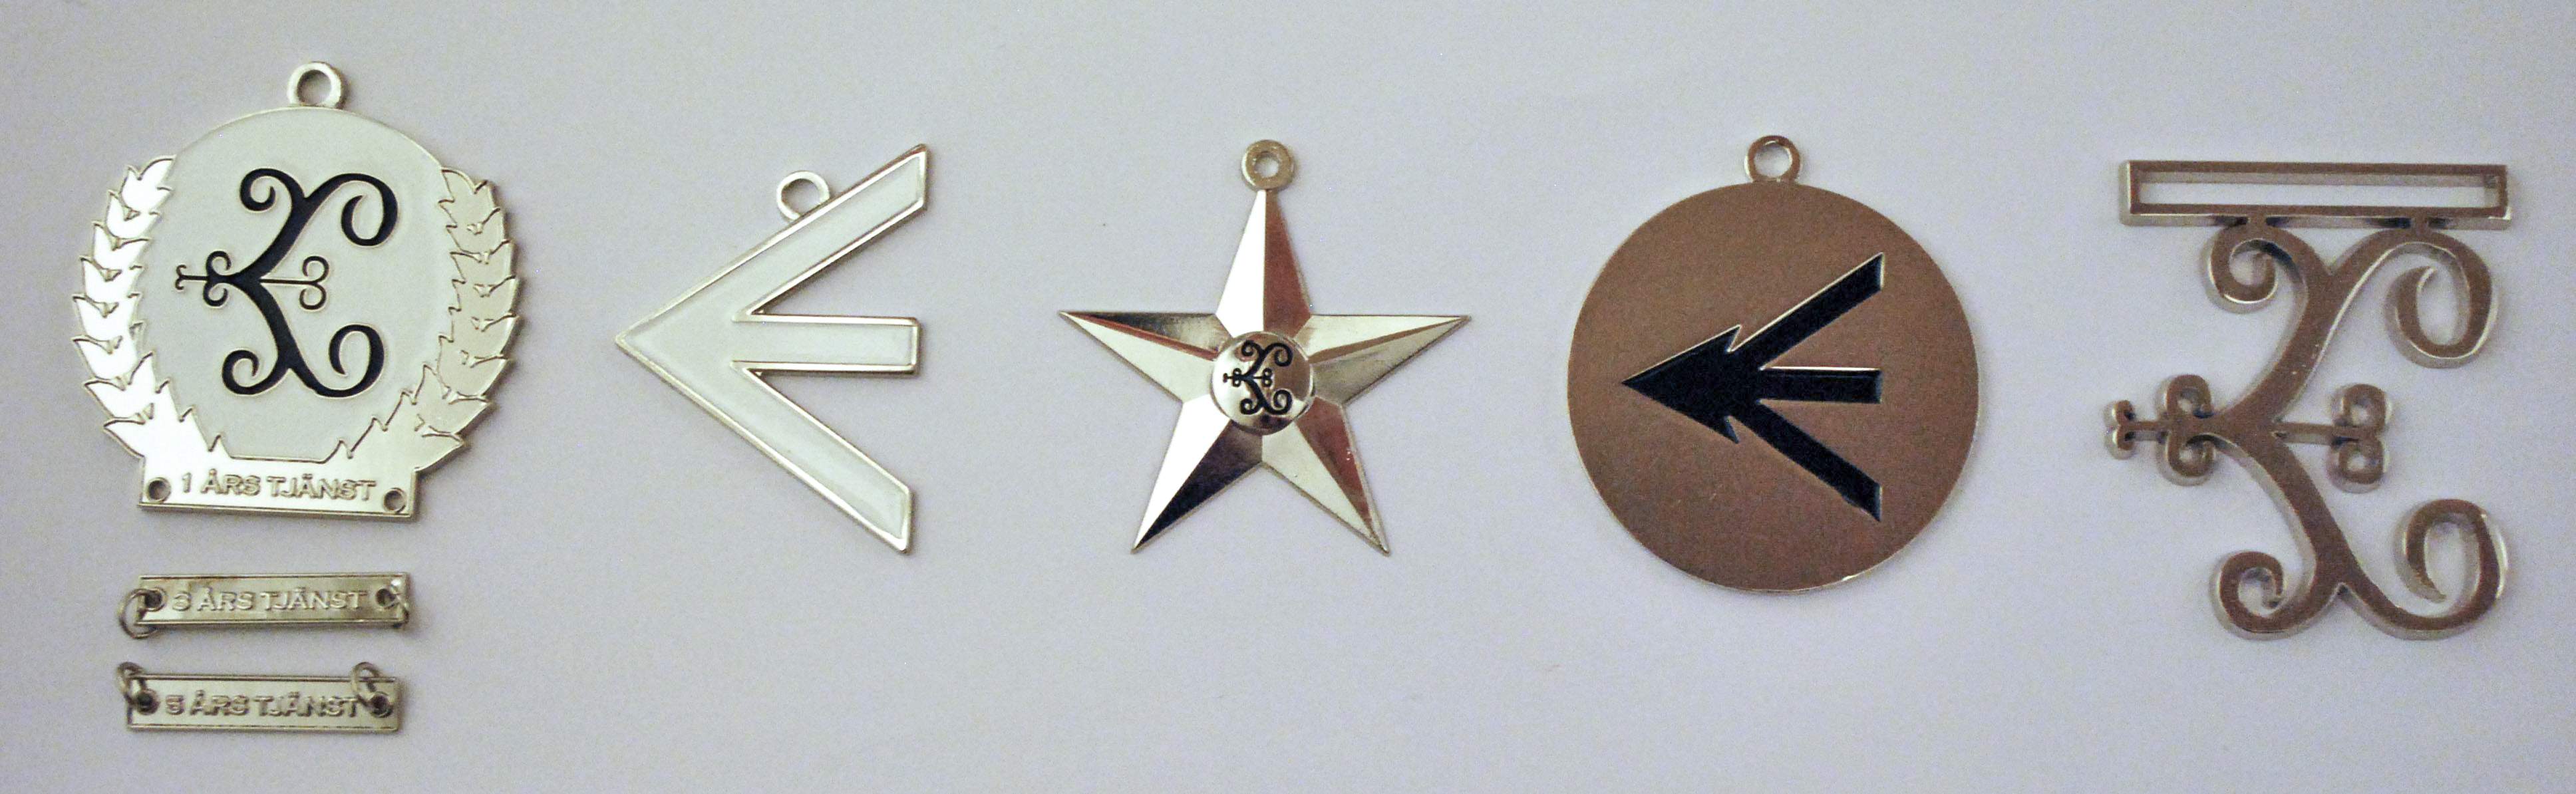
\includegraphics[width=0.9\textwidth]{pol_medaljer.jpg}\\
\end{center}
{Sektionens medaljer. Från vänster: Funktionärsmedalj 1 år med tillägg för 3 samt 5 år, Styrelsemedalj, Bidragsmedalj, Utomstående Förtjänstmedalj samt Krusidull-E.}
\end{figure}

\changenote


\end{document}
